%% triple-diff.tex — Zurich Day 2 (morning): Triple Differences
%% Scott Cunningham, University of Zurich, May 12, 2026
%%
%% Compile: pdflatex triple-diff.tex
%% Style:   remix.sty (in same directory)
%%
%% Pedagogical structure: problem -> narrative -> picture -> codeblock -> intuition -> technical
%% Source material: heavy copy from
%%   /Users/scunning/Causal-Inference-2/Slides/Tex/02-Codechella-Violations.tex
%%   /Users/scunning/Causal-Inference-2/Lab/DDD/ddd2.R (ported to decks/code/Triple-Diff/)

\documentclass[aspectratio=169,11pt]{beamer}
\usepackage{remix}

\usepackage{tikz}
\usetikzlibrary{positioning,arrows.meta,calc,shapes.geometric,fit,backgrounds}
\usepackage{listings}
\usepackage{xcolor}
\usepackage{booktabs}
\usepackage{colortbl}

\tikzset{
  trendline/.style={line width=1pt, accent},
  trendcontrol/.style={line width=1pt, slate, dashed},
}

\lstset{
  basicstyle=\ttfamily\footnotesize,
  keywordstyle=\color{accentdark}\bfseries,
  commentstyle=\color{warmgray}\itshape,
  stringstyle=\color{ocean},
  backgroundcolor=\color{lightbg},
  frame=single,
  framesep=4pt,
  rulecolor=\color{warmgray!40},
  columns=fullflexible,
  showstringspaces=false,
  breaklines=true,
  numbers=none,
  xleftmargin=0.4em,
  xrightmargin=0.4em,
}

\renewcommand{\remixfooter}{University of Zurich\,\textperiodcentered\,Department of Economics\,\textperiodcentered\,May 2026}

\begin{document}

%% =====================================================================
%%                                ACT I
%% =====================================================================

%% ---------- Slide 1: TITLE ----------
\remixtitleframe
  {Triple Differences}
  {Day 2 of 3, Morning: When parallel trends fails, find a third group}
  {Scott Cunningham \textperiodcentered\ Baylor University}
  {University of Zurich \textperiodcentered\ May 12, 2026}

%% ---------- Slide 2: Where we are ----------
\begin{frame}{Yesterday's closing claim, today's tension}
\vspace{0.6em}
\pullquote{DiD is a research design with two ingredients --- the 2$\times$2 calculation and parallel trends --- and together they identify the ATT.}{Day 1 closing slide}
\vspace{0.6em}
\begin{itemize}
  \item Yesterday: \highlight{if you believe PT, the 2$\times$2 identifies the ATT.}
  \item Today: \highlight{what if you don't believe PT?}
  \item Two answers --- both responses to a PT violation. This morning: \highlight{a third group}. This afternoon: \highlight{covariates}.
\end{itemize}
\end{frame}

%% ---------- Slide 3: The applied problem ----------
\begin{frame}{The applied problem}
\vspace{0.5em}
You think a state's policy moved an outcome. You build the 2$\times$2:
\vspace{0.3em}
\begin{center}
\small
$\widehat{\delta}_{2\times 2} = (\overline{Y}^{TX}_{\text{post}} - \overline{Y}^{TX}_{\text{pre}}) - (\overline{Y}^{AR}_{\text{post}} - \overline{Y}^{AR}_{\text{pre}})$
\end{center}
\vspace{0.4em}
\begin{itemize}
  \item But you suspect Texas was already on a different trajectory --- for reasons unrelated to the policy.
  \item PT is violated. The 2$\times$2 is biased. \highlight{Now what?}
  \item One option: find a group inside Texas that experiences \textit{the same trend bias} but is NOT subject to the policy. Subtract their bias off.
  \item That move is the \highlight{triple difference}.
\end{itemize}
\end{frame}

%% ---------- Slide 4: Today's seven beats ----------
\begin{frame}{This morning, six beats}
\vspace{0.4em}
\begin{enumerate}
  \item Gruber 1994: the canonical DDD application
  \item Two biased DiDs --- and one parallel-bias assumption
  \item The 8-cell calculation, by hand
  \item A simulation: see the bias, see DDD recover the ATT
  \item DDD as a regression specification
  \item When DDD goes wrong --- and Gruber's actual numbers
\end{enumerate}
\end{frame}

%% =====================================================================
%%                                LESSON 1
%% =====================================================================
\remixsection{1.\ Gruber and the Maternity Mandate}

%% ---------- L1-F1: the policy ----------
\begin{frame}{The policy: 1976 maternity insurance mandates}
\vspace{0.4em}
\begin{itemize}
  \item Several states in 1976 mandated that employer-provided health insurance cover \textit{childbirth on the same terms as any other medical condition}.
  \item Before: pregnancy could be excluded from coverage.
  \item Cost to insurers $\rightarrow$ cost to employers $\rightarrow$ \highlight{cost to whom?}
\end{itemize}
\vspace{0.5em}
\begin{block}{The economic question}
\small
Did the burden shift back to childbearing-age women in the form of \highlight{lower wages}? Or did employers absorb it? Or was it shifted to consumers?
\end{block}
\end{frame}

%% ---------- L1-F2: who pays ----------
\begin{frame}{Whose wages would have to fall?}
\vspace{0.4em}
If the mandate truly raises the employment cost of childbearing-age women, classical incidence reasoning predicts the cost shifts to \textit{them} via lower wages.
\vspace{0.6em}
\begin{itemize}
  \item Treated cell: \highlight{married women 20--40} in mandate states.
  \item Comparison group --- naive: married women 20--40 in non-mandate states.
  \item But: women's labor-market outcomes were diverging across states for many reasons (manufacturing decline, services growth, two-earner-household norms). \highlight{PT is suspect.}
\end{itemize}
\end{frame}

%% ---------- L1-F3: Gruber's move ----------
\begin{frame}{Gruber's move: bring in a third group}
\vspace{0.4em}
\begin{itemize}
  \item In the same state, in the same labor market, take a group the mandate \textit{should not touch}: \highlight{single men and older women.}
  \item They live in the same economy. The same trends hit them.
  \item But they're not the ones the mandate raised the cost of employing.
\end{itemize}
\vspace{0.6em}
\begin{block}{The bet}
\small
If the differential state trend hits the treated group AND the placebo group equally hard, the placebo group's ``DiD'' just \textit{is} the bias. \\[0.2em]
\highlight{Subtract the placebo DiD from the naive DiD --- get the ATT.}
\end{block}
\end{frame}

%% =====================================================================
%%                                LESSON 2
%% =====================================================================
\remixsection{2.\ Two Biased DiDs, One Bias}

%% ---------- L2-F1: the biased DiD ----------
\begin{frame}{Biased DiD \#1 --- married women, two states}
\vspace{0.4em}
\begin{center}
\small
\renewcommand{\arraystretch}{1.3}
\begin{tabular}{@{}lcc@{}}
\toprule
 & \textbf{Mandate states (NJ)} & \textbf{Control states (PA)} \\
\midrule
Pre  & $Y = NJ$                          & $Y = PA$        \\
Post & $Y = NJ + NJ_t + D$               & $Y = PA + PA_t$ \\
\midrule
\textit{Difference (post-pre)} & $NJ_t + D$ & $PA_t$ \\
\bottomrule
\end{tabular}
\end{center}
\vspace{0.5em}
\[
\widehat{\delta}_{\text{DiD}} \;=\; (NJ_t + D) - PA_t \;=\; D \;+\; \underbrace{(\textcolor{accent}{NJ_t} - PA_t)}_{\textstyle\text{bias if } \textcolor{accent}{NJ_t} \neq PA_t}
\]
\vspace{0.1em}
The naive DiD recovers the ATT \textit{only if} the state trends were the same. \highlight{Assume they aren't.}
\end{frame}

%% ---------- L2-F2: the placebo DiD ----------
\begin{frame}{Biased DiD \#2 --- single men + older women, same two states}
\vspace{0.4em}
\begin{center}
\small
\renewcommand{\arraystretch}{1.3}
\begin{tabular}{@{}lcc@{}}
\toprule
 & \textbf{Mandate states (NJ)} & \textbf{Control states (PA)} \\
\midrule
Pre  & $Y = NJ$        & $Y = PA$        \\
Post & $Y = NJ + NJ_t$ & $Y = PA + PA_t$ \\
\midrule
\textit{Difference (post-pre)} & $NJ_t$ & $PA_t$ \\
\bottomrule
\end{tabular}
\end{center}
\vspace{0.5em}
\[
\widehat{\delta}^{\text{placebo}}_{\text{DiD}} \;=\; NJ_t - PA_t \;=\; \textcolor{accent}{NJ_t - PA_t}
\]
\vspace{0.1em}
No treatment here. The placebo DiD \textit{is} the bias --- nothing else.
\end{frame}

%% ---------- L2-F3: the subtraction ----------
\begin{frame}{Subtract the bias --- triple difference}
\vspace{0.4em}
\[
\widehat{\delta}_{\text{DDD}} \;=\; \widehat{\delta}_{\text{DiD}} \;-\; \widehat{\delta}^{\text{placebo}}_{\text{DiD}}
\]
\vspace{-0.2em}
\[
= \big[D + (NJ_t - PA_t)\big] \;-\; (NJ_t - PA_t) \;=\; D
\]
\vspace{0.3em}
\begin{block}{The new identifying assumption: \highlight{parallel bias}}
\small
\centering
$(NJ_t - PA_t)^{\text{married}} \;=\; (NJ_t - PA_t)^{\text{placebo}}$
\end{block}
\vspace{0.4em}
\begin{itemize}\small
  \item \textbf{Not} ``two parallel trends.'' One assumption: the \textit{differential} state trend hits both groups the same.
  \item Trends can differ. Levels can differ. The cross-state \textit{gap} in trends has to be the same across the two demographic groups.
\end{itemize}
\end{frame}

%% ---------- L2-F4: Olden & Møen formal version ----------
\begin{frame}{The formal version --- Olden \& Møen (2022)}
\vspace{0.3em}
{\footnotesize Same idea, in potential-outcomes form:}
\vspace{-0.2em}
\[
\underbrace{E[\Delta Y^0 \mid D=1, G=1] - E[\Delta Y^0 \mid D=0, G=1]}_{\text{bias in the main DiD (eligible group)}}
\]
\vspace{-0.6em}
\[
=
\]
\vspace{-0.6em}
\[
\underbrace{E[\Delta Y^0 \mid D=1, G=0] - E[\Delta Y^0 \mid D=0, G=0]}_{\text{bias in the placebo DiD (ineligible group)}}
\]
\vspace{0.2em}
\begin{itemize}\small
  \item $D$: treatment state. \;$G$: eligible group. \;$\Delta Y^0$: change in the \textit{untreated} potential outcome.
  \item Each component DiD has its own non-parallel-trends bias.
  \item DDD identifies the ATT iff the two biases are \highlight{equal} --- not zero.
\end{itemize}
\vspace{0.2em}
\meta{Olden \& Møen (2022), \textit{Econometrics Journal} 25(3). They call it the \textit{bias stability} assumption (after Fr{\"o}lich \& Sperlich 2019).}
\end{frame}

%% ---------- L2-F5: my own footnote — the credibility move ----------
\begin{frame}{A pedagogical aside: I got it slightly wrong}
\vspace{0.3em}
\begin{itemize}
  \item In the \textit{Mixtape} 1st edition, I stated the DDD identifying assumption \textit{verbally} --- and imprecisely.
  \item Olden \& Møen (2022) wrote down the first formal statement (above).
  \item The 2nd edition (Yale UP, 2026) now carries their equation, with a footnote crediting them and quoting my earlier imprecise version.
\end{itemize}
\vspace{0.5em}
\begin{block}{Why I'm telling you this}
\small
DDD has been used in top journals since Gruber (1994) --- yet for nearly three decades nobody had written down its identifying assumption in expectations. The literature ran on intuition. \\[0.3em]
\highlight{Method papers fill quiet gaps. Read them.}
\end{block}
\end{frame}

%% ---------- L2-F6: design vs falsification ----------
\begin{frame}{DDD is a design, not a falsification}
\vspace{0.4em}
\begin{itemize}
  \item A \highlight{design} has an identifying assumption. \;The assumption is what delivers the estimate.
  \item A \highlight{falsification} is a test or a conjecture --- a probe of whether some \textit{other} design's assumption is credible.
\end{itemize}
\vspace{0.6em}
\begin{block}{Same procedure, different jobs}
\small
\textit{Placebo DiD as falsification}: run DiD on a group whose outcome shouldn't move. If it doesn't, your original DiD's parallel trend looks credible. \;That's a \textit{check on DiD}. \\[0.3em]
\textit{Placebo DiD as DDD}: subtract the placebo DiD from the main DiD. The difference \textit{is} the estimate. \;That's a \textit{new design}, with its own assumption (parallel bias).
\end{block}
\vspace{0.3em}
\meta{The arithmetic looks identical. The interpretation is not. Identifying assumption $\Rightarrow$ design; conjecture $\Rightarrow$ falsification.}
\end{frame}

%% =====================================================================
%%                                LESSON 3
%% =====================================================================
\remixsection{3.\ The 8 Cells}

%% ---------- L3-F1: the cube ----------
\begin{frame}{The DDD cube --- two states $\times$ two periods $\times$ two groups}
\vspace{0.3em}
\begin{center}
\begin{tikzpicture}[scale=0.85, every node/.style={font=\small}]
  % Front face: mandate states, married women
  \fill[remixgreenlight] (0,0) rectangle (2,1.5);
  \fill[remixgreenlight] (2,0) rectangle (4,1.5);
  \fill[lightbg]         (0,1.5) rectangle (2,3);
  \fill[lightbg]         (2,1.5) rectangle (4,3);
  \draw[charcoal, thin] (0,0) rectangle (4,3);
  \draw[charcoal, thin] (2,0) -- (2,3);
  \draw[charcoal, thin] (0,1.5) -- (4,1.5);

  % Back face: control states, married women (offset behind)
  \fill[white, opacity=0.6] (1,0.7) rectangle (5,3.7);
  \draw[charcoal, thin, opacity=0.6] (1,0.7) rectangle (5,3.7);
  \draw[charcoal, thin, opacity=0.6] (3,0.7) -- (3,3.7);
  \draw[charcoal, thin, opacity=0.6] (1,2.2) -- (5,2.2);

  % Connecting edges
  \draw[charcoal, thin, opacity=0.5] (0,0) -- (1,0.7);
  \draw[charcoal, thin, opacity=0.5] (4,0) -- (5,0.7);
  \draw[charcoal, thin, opacity=0.5] (0,3) -- (1,3.7);
  \draw[charcoal, thin, opacity=0.5] (4,3) -- (5,3.7);

  % Labels
  \node[font=\scriptsize, anchor=south, text=charcoal] at (2,3.2) {Pre $\;\;\;\;\;$ Post};
  \node[font=\scriptsize, anchor=east,  text=charcoal] at (-0.1, 0.75) {Married};
  \node[font=\scriptsize, anchor=east,  text=charcoal] at (-0.1, 2.25) {Placebo};
  \node[font=\scriptsize, anchor=west,  text=accent]   at (4.1, 1.5) {Mandate states};
  \node[font=\scriptsize, anchor=west,  text=slate]    at (5.1, 2.2) {Control states};

  % Center label
  \node[font=\scriptsize\itshape, text=charcoal] at (2,-0.6) {8 cells: states $\times$ groups $\times$ periods};
\end{tikzpicture}
\end{center}
\vspace{0.6em}
\begin{center}
\footnotesize\color{warmgray}\itshape
We need 8 averages. We will form 3 subtractions twice over --- a 2$\times$2 DiD for each group --- then subtract the placebo DiD from the treated DiD. One number.
\end{center}
\end{frame}

%% ---------- L3-F2: the 8 cells table ----------
\begin{frame}{The 8 cells, filled in from the simulation}
\vspace{0.4em}
\begin{center}
\footnotesize
% Auto-generated by ddd_simulation.R -- do not hand-edit
\begin{tabular}{@{}lcccc@{}}
\toprule
 & \multicolumn{2}{c}{\textbf{Mandate states}} & \multicolumn{2}{c}{\textbf{Control states}} \\
\cmidrule(lr){2-3}\cmidrule(lr){4-5}
 & Pre & Post & Pre & Post \\
\midrule
Married women 20--40        & 70,503 & 73,813 & 49,006 & 60,013 \\
Placebo (men + older women) & 71,510 & 82,490 & 50,003 & 63,742 \\
\bottomrule
\end{tabular}

\end{center}
\vspace{0.6em}
\begin{itemize}\small
  \item \textbf{Naive DiD} (married women): $(\$57{,}488 - \$58{,}722) - (\$70{,}224 - \$66{,}760) \approx -\$7{,}697$
  \item \textbf{Placebo DiD} (men + older women): $\approx -\$2{,}759$
  \item \textbf{DDD}: $-\$7{,}697 \;-\; (-\$2{,}759) \;=\; \mathbf{-\$4{,}938}$
\end{itemize}
\vspace{0.3em}
\begin{center}
\small\color{warmgray}\itshape
True ATT in the simulation: $-\$5{,}000$. DDD recovers it. Naive DiD is off by 54\%.
\end{center}
\meta{Simulation: \texttt{zurich/labs/Triple-Diff/ddd\_simulation.R}. \;40 states $\times$ 50 cities $\times$ 3 worker groups $\times$ 11 years; seed 20200403.}
\end{frame}

%% ---------- L3-F3: DDD formula ----------
\begin{frame}{The DDD formula --- one line, eight cells}
\vspace{0.6em}
\begin{center}
\small
$\widehat{\delta}_{\text{DDD}} = \big[(\overline{Y}^{TX,M}_1 - \overline{Y}^{TX,M}_0) - (\overline{Y}^{AR,M}_1 - \overline{Y}^{AR,M}_0)\big]$\\[0.4em]
$\hspace{2.5em} - \;\big[(\overline{Y}^{TX,P}_1 - \overline{Y}^{TX,P}_0) - (\overline{Y}^{AR,P}_1 - \overline{Y}^{AR,P}_0)\big]$
\end{center}
\vspace{0.7em}
\begin{itemize}\small
  \item Superscripts: state (TX = mandate, AR = control), group (M = married, P = placebo)
  \item Subscripts: 0 = pre, 1 = post
  \item Read it as: \highlight{(DiD for the treated group)} minus \highlight{(DiD for the placebo group)}.
  \item Two DiDs. One subtraction. That is all.
\end{itemize}
\end{frame}

%% =====================================================================
%%                                LESSON 4
%% =====================================================================
\remixsection{4.\ A Simulation Makes It Visible}

%% ---------- L4-F1: see the trends ----------
\begin{frame}{See the bias before you read the regression}
\vspace{-0.2em}
\begin{center}
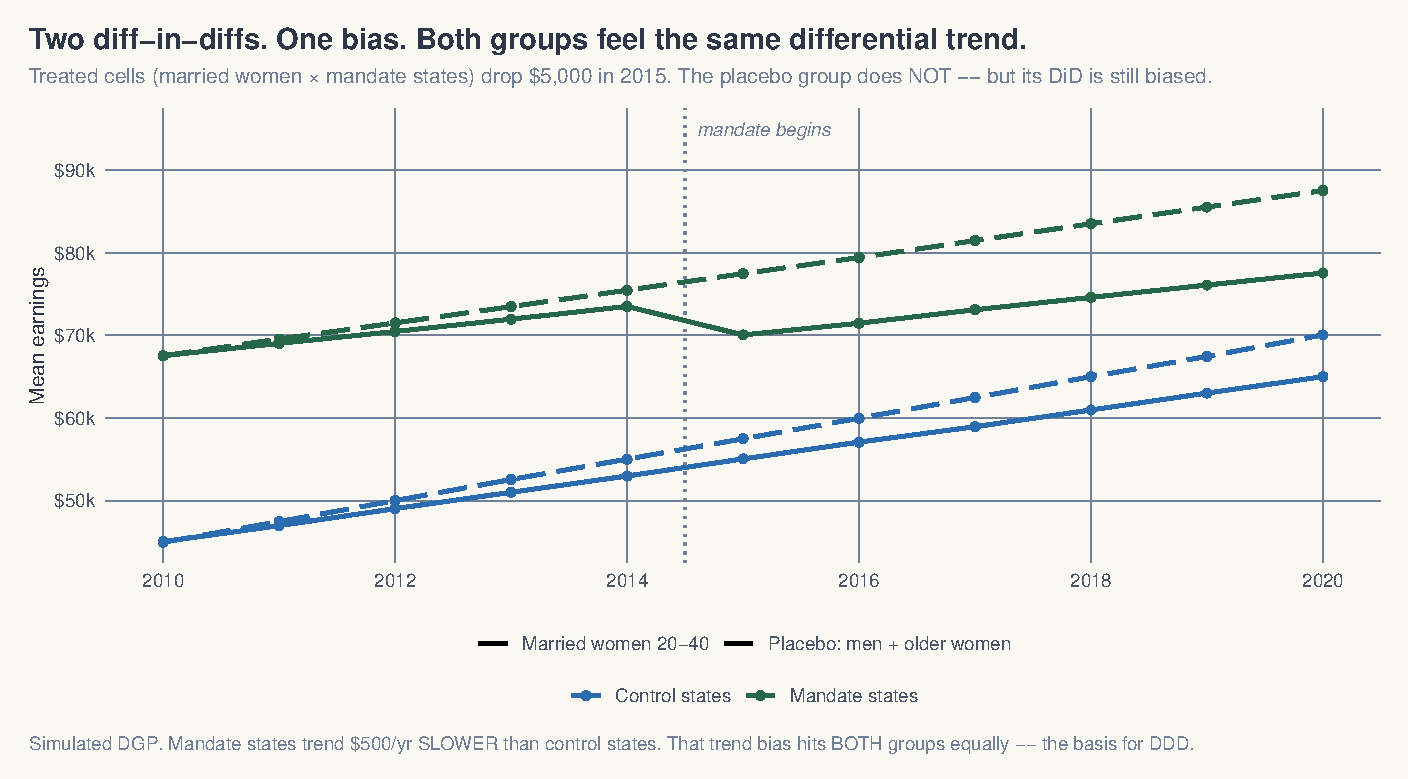
\includegraphics[width=0.94\linewidth,height=0.72\textheight,keepaspectratio]{figures/triple_diff_trends.pdf}
\end{center}
\vspace{-0.4em}
\begin{center}
\footnotesize\color{warmgray}\itshape
Mandate states (green) trend slower than control states (blue) --- for BOTH groups. \\
That's the bias. The placebo group is in the same economy --- it feels the same shift.
\end{center}
\end{frame}

%% ---------- L4-F2: codeblock ----------
\begin{frame}[fragile]{The simulation, code first}
\vspace{0.2em}
\begin{lstlisting}[language=R]
# DGP knobs:
#   40 states (1-20 mandate, 21-40 control)
#   3 worker groups (men, married women 20-40, older women)
#   2010-2020; treatment turns on in 2015
#   TRUE ATT for married x mandate x post = -$5,000

df$state_trend <- if_else(df$experimental==1, 1000, 1500)  # !! differential
df$group_trend <- if_else(df$worker==2,       500, 1000)
df$y0 <- df$baseline +
         df$state_trend * df$year_diff +
         df$group_trend * df$year_diff + rnorm(N, 0, 1500)

df$treat    <- (df$experimental==1 & df$worker==2 & df$after==1)
df$y1       <- df$y0 - 5000 * df$treat
df$earnings <- df$treat * df$y1 + (1-df$treat) * df$y0
\end{lstlisting}
\vspace{0.2em}
\meta{Full script: \texttt{decks/code/Triple-Diff/ddd\_simulation.R}}
\end{frame}

%% ---------- L4-F3: event study ----------
\begin{frame}{Three event studies, one figure}
\vspace{-0.2em}
\begin{center}
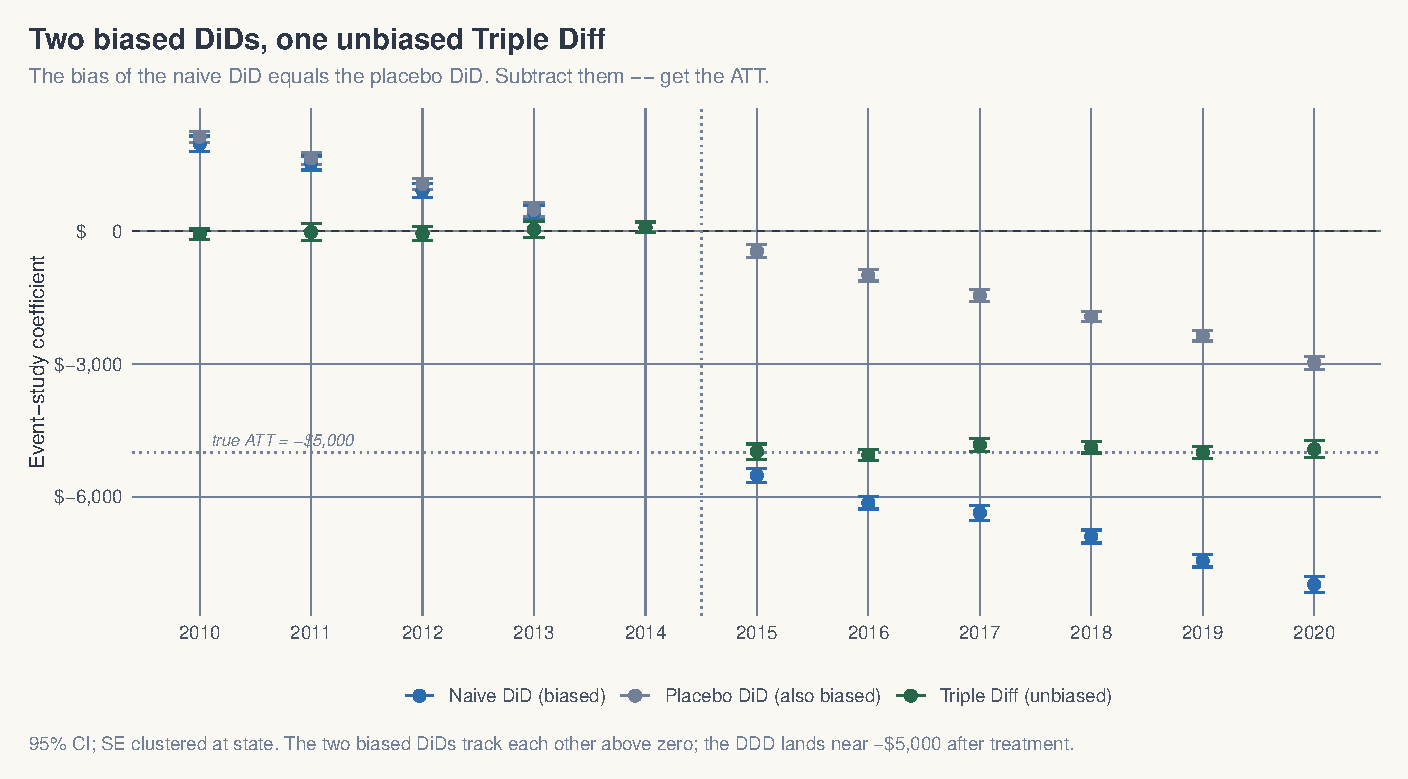
\includegraphics[width=0.92\linewidth,height=0.72\textheight,keepaspectratio]{figures/triple_diff_eventstudy.pdf}
\end{center}
\vspace{-0.3em}
\begin{center}
\footnotesize\color{warmgray}\itshape
Naive DiD (blue) lands too negative. Placebo DiD (gray) is the bias --- nonzero even though nothing happened. \\
\highlight{Triple Diff (green) lands at the true ATT of $-\$5{,}000$.}
\end{center}
\end{frame}

%% =====================================================================
%%                                LESSON 5
%% =====================================================================
\remixsection{5.\ DDD as a Regression}

%% ---------- L5-F1: the saturated regression ----------
\begin{frame}{The saturated triple-interaction regression}
\vspace{0.4em}
\small
\begin{align*}
Y_{ijt} \;=\;& \alpha
            + \beta_1 D_i
            + \beta_2 G_j
            + \beta_3 \tau_t
            + \beta_4 (D_i \times G_j)
            + \beta_5 (D_i \times \tau_t) \\
            &+ \beta_6 (G_j \times \tau_t)
            + \;\textcolor{accent}{\boldsymbol{\delta} \,(D_i \times G_j \times \tau_t)}
            + \varepsilon_{ijt}
\end{align*}
\vspace{0.2em}
\begin{itemize}\small
  \item $D_i$: state is a mandate state. \;\; $G_j$: worker is in the treated group (married women 20--40). \;\; $\tau_t$: post-period.
  \item \highlight{$\boldsymbol{\delta}$} is the triple interaction --- the DDD estimate of the ATT.
  \item Every two-way interaction is also there. The triple strips out everything but the answer.
\end{itemize}
\end{frame}

%% ---------- L5-F2: identifying assumptions ----------
\begin{frame}{What the regression assumes}
\vspace{0.4em}
\begin{itemize}
  \item \textbf{Parallel bias}: the differential state-trend that biases the treated DiD biases the placebo DiD by \textit{the same amount}.
  \item \textbf{No anticipation}: the treated group didn't shift behavior before $t = 2015$.
  \item \textbf{SUTVA}: one unit's treatment doesn't change another unit's $Y(0)$.
\end{itemize}
\vspace{0.6em}
\begin{block}{What DDD does \textit{not} require}
\small
\textit{Two} parallel-trends assumptions (one per group). That misconception --- DDD as a ``double check'' --- is wrong. \\[0.2em]
DDD has \textit{one} identifying assumption, and it's weaker than the DiD's. That's its appeal.
\end{block}
\end{frame}

%% =====================================================================
%%                                LESSON 6
%% =====================================================================
\remixsection{6.\ Caveats, Gruber's Actual Numbers, \\[0.3em] and When DDD Goes Wrong}

%% ---------- L6-F1a: Gruber's actual numbers, the table ----------
\begin{frame}{Gruber (1994): the actual numbers (log hourly wages)}
\begin{center}
\renewcommand{\arraystretch}{1.0}
\scriptsize
\begin{tabular}{@{}lccc@{}}
\toprule
\textbf{Location / year}                 & \textbf{Pre-law} & \textbf{Post-law} & \textbf{Difference} \\
\midrule
\multicolumn{4}{l}{\textit{A. Treatment: Married women 20--40}} \\
\;\;Experimental states                  & 1.547 (.012)     & 1.513 (.012)      & $-$0.034 (.017) \\
\;\;Control states                       & 1.369 (.010)     & 1.397 (.010)      & $+$0.028 (.014) \\
\;\;\textbf{DiD (A)}                     &                  &                   & \cellcolor{remixgreenlight}$\mathbf{-0.062}$ (.022) \\
\midrule
\multicolumn{4}{l}{\textit{B. Placebo: Over 40 + Single Males 20--40}} \\
\;\;Experimental states                  & 1.759 (.007)     & 1.748 (.007)      & $-$0.011 (.010) \\
\;\;Control states                       & 1.630 (.007)     & 1.627 (.007)      & $-$0.003 (.010) \\
\;\;\textbf{DiD (B, placebo)}            &                  &                   & \cellcolor{remixgreenlight}$\mathbf{-0.008}$ (.014) \\
\midrule
\multicolumn{3}{r}{\textbf{DDD = (A) $-$ (B) $\;=\;$}} & \cellcolor{remixgreenlight}$\mathbf{-0.054}$ (.026) \\
\bottomrule
\end{tabular}
\end{center}
\vspace{0.3em}
{\footnotesize DDD $=$ True DiD $-$ Placebo DiD. Placebo DiD $= -0.008$ --- essentially zero, so the original DD ($-0.062$) was already approximately unbiased. DDD and DD agree because there was no differential trend to subtract.}
\meta{Source: Gruber (1994) AER. Reproduced in Cunningham, \textit{Mixtape} \S 9.}
\end{frame}

%% ---------- L6-F1b: The honest interpretive frame ----------
\begin{frame}{What this means for when DDD ``mattered''}
\vspace{0.5em}
\begin{itemize}
  \item Gruber's naive DiD: \;\;\;\highlight{$-6.2\%$} \\
        Gruber's triple diff: \highlight{$-5.4\%$} \\
        Very close. \;\textit{Was DDD necessary?}
  \item In this case, no. The placebo wage trend was essentially zero, so the DD was already approximately unbiased.
  \item But that's the wrong question.
\end{itemize}
\vspace{0.5em}
\begin{block}{The honest answer}
\small
\highlight{The value of DDD is what it would have caught.} \;The placebo DiD was a real opportunity to invalidate the design. It didn't. The design is more credible because it \textit{could have} failed.
\end{block}
\vspace{0.2em}
\meta{This is the Popper move from Day 1, in a different costume.}
\end{frame}

%% ---------- L6-F2: when DDD goes wrong ----------
\begin{frame}{When DDD is worse than DiD}
\vspace{0.4em}
\begin{itemize}\small
  \item \textbf{The placebo group is also treated} --- by a different policy that hit at the same time. Now the placebo DiD reflects \textit{that} policy, and subtracting it injects bias instead of removing it.
  \item \textbf{The bias is not common} --- the differential state-trend hits the treated group but not the placebo group (or hits with a different magnitude). DDD identifies a parameter you didn't want.
  \item \textbf{Wrong placebo group} --- one that experiences the policy through indirect channels. Subtracting it removes signal, not bias.
\end{itemize}
\vspace{0.5em}
\begin{center}
\small\color{warmgray}\itshape
The first defense is the placebo-group event study. If the placebo group has its own discontinuity at the treatment date, the placebo isn't placebo.
\end{center}
\end{frame}

%% ---------- L6-F3: the ladder of evidence ----------
\begin{frame}{Even DDD wants its event study}
\vspace{0.4em}
\begin{itemize}
  \item DDD is a design, not a black box. You owe the reader the same five pieces from Day 1:
  \begin{itemize}\small
    \item[--] \textbf{Bite}: did the policy bind?
    \item[--] \textbf{Event study}: pre-trends on the DDD coefficient (we built one --- show it)
    \item[--] \textbf{Falsification}: a placebo for the \textit{placebo group} itself
    \item[--] \textbf{Main result}: the DDD point estimate
    \item[--] \textbf{Mechanism}: the channel from policy to outcome
  \end{itemize}
  \item \highlight{The event study is the way you defend parallel bias.} Plot it. Show that pre-period DDD coefficients are flat. Then the post-period estimate is credible.
\end{itemize}
\end{frame}

%% =====================================================================
%%                                ACT III
%% =====================================================================

%% ---------- Recap ----------
\begin{frame}{What we've done this morning}
\vspace{0.3em}
\begin{enumerate}
  \item Gruber 1994: a maternity-benefit story that DiD couldn't tell
  \item Two biased DiDs $\rightarrow$ one bias $\rightarrow$ subtract
  \item The 8 cells, by hand, with the simulation matching
  \item A picture showing parallel bias in trends
  \item DDD as the saturated triple-interaction regression
  \item One identifying assumption, not two --- and how it fails
\end{enumerate}
\end{frame}

%% ---------- Lab: triple-diff on Scott's abortion data ----------
\begin{frame}{Lab over lunch: abortion legalization \& gonorrhea (3$\times$2)}
\vspace{0.3em}
\textbf{Goal.} Take the DDD machinery and run it on data Scott actually published with.
\vspace{0.4em}
\begin{itemize}\small
  \item Cunningham \& Cornwell (2013), in the lineage of Donohue \& Levitt (2001). \;\highlight{Treated cohort:} Black females 15--19 (\texttt{bf15}). \;\highlight{Placebo cohort:} Black females 25--29 (\texttt{bf25}).
  \item Repeal states vs.\ Roe states; \;pre/post the affected birth cohort. \;Eight cells.
  \item \textbf{Part 1:} compute the 8 cell means and the DDD by hand (weighted by \texttt{totpop}).
  \item \textbf{Part 2:} recover the same number via \texttt{lnr $\sim$ repeal\#cohort\_treated\#post}, clustered at \texttt{fip}.
  \item \textbf{Part 3:} compare hand vs.\ regression; check what happens if you cluster wrong.
  \item \textbf{Part 4:} write a paragraph on what the placebo cohort buys you over Donohue \& Levitt's straight DD.
\end{itemize}
\vspace{0.4em}
\meta{Walkthrough: \texttt{zurich/labs/Triple-Diff/README.md}. \;Data: \texttt{abortion.dta} on Scott's GitHub.}
\end{frame}

%% ---------- Bridge ----------
\begin{frame}{This afternoon}
\vspace{0.4em}
\begin{itemize}
  \item DDD's escape hatch needs a \highlight{third group} that shares the bias.
  \item Often you don't have one.
  \item Then the move is: \highlight{condition on covariates}. Inverse propensity weighting, outcome regression, doubly robust.
  \item And one false friend: \textit{controlling for the propensity score in a regression}. That's not what DR is. We'll see why.
\end{itemize}
\end{frame}

%% ---------- Closing one-sentence linger ----------
\begin{frame}[plain]
\begin{tikzpicture}[remember picture,overlay]
\fill[cream] (current page.south west) rectangle (current page.north east);
\node[anchor=center, text width=0.82\paperwidth, align=center, text=charcoal] at (current page.center) {%
  \fontsize{22pt}{30pt}\selectfont
  Triple diff trades parallel trends\\[0.4em]
  for {\color{accent}\bfseries parallel bias.}
};
\draw[accent, line width=1pt] ([yshift=1.8cm,xshift=0.25\paperwidth]current page.south west) -- ([yshift=1.8cm,xshift=-0.25\paperwidth]current page.south east);
\node[anchor=south] at ([yshift=0.7cm]current page.south) {%
  \color{warmgray}\fontsize{10pt}{12pt}\selectfont \textit{Back after lunch --- covariates.}
};
\end{tikzpicture}
\end{frame}

\end{document}
